



\begin{figure}[tb]
	\begin{center}
		\vspace{-.2in}
		
		\begin{tabular}{   c c | c  c  c   }
			%\hline
			& & \large{\textsf{23 GST}} &\large{\textsf{2 GST}}   &\large{\textsf{6 GST}}    \\ 
			&\vspace{-.1in} & & & \\ \hline
			&\vspace{-.1in} & & & \\
			& \multirow{1}{*}[0.45in]{ \rotatebox[origin=t]{90}{\small{\textsf{Truth}} }} & 
			{{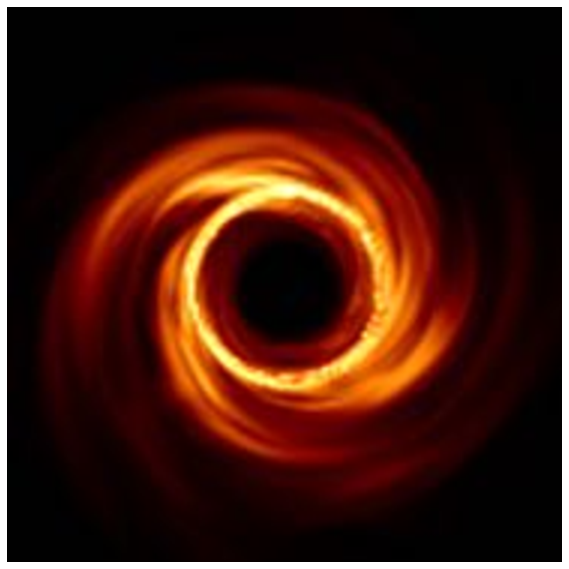
\includegraphics[height=.2\linewidth]{figures/propcmp/gt/gt_74.pdf}} } &
			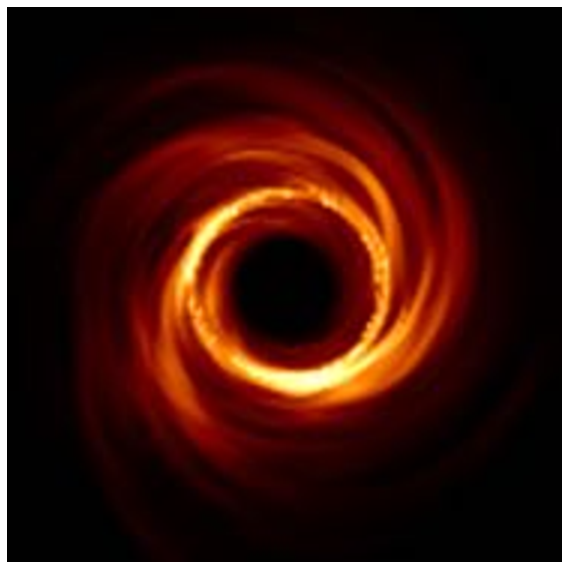
\includegraphics[height=.2\linewidth]{figures/propcmp/gt/gt_111.pdf} &
			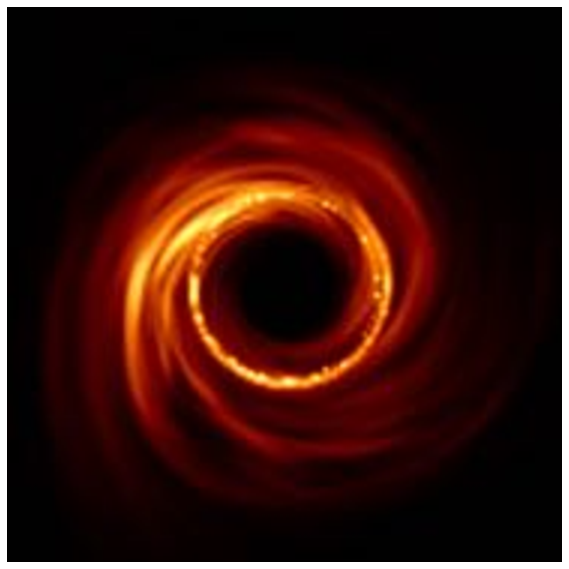
\includegraphics[height=.2\linewidth]{figures/propcmp/gt/gt_159.pdf}  
			\\ \hline
			&\vspace{-.1in} & & & \\
			\multirow{1}{*}[0.6in]{ \rotatebox[origin=t]{90}{\small{\textsf{NO ATM. \& }} }} \hspace{-0.25in} &
			\multirow{1}{*}[0.55in]{ \rotatebox[origin=t]{90}{\small{\textsf{ NO PROP.}} }} &
			{{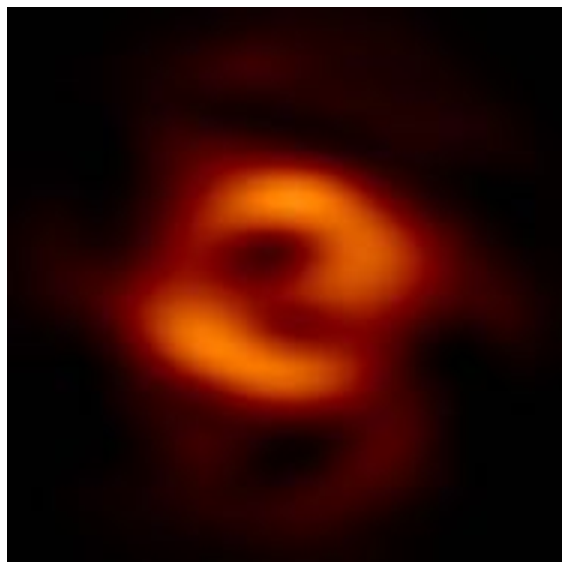
\includegraphics[height=.2\linewidth]{figures/propcmp/nomotion_NOPROP_hotoka02_vis_eht2017/mean_74.pdf}} } &
			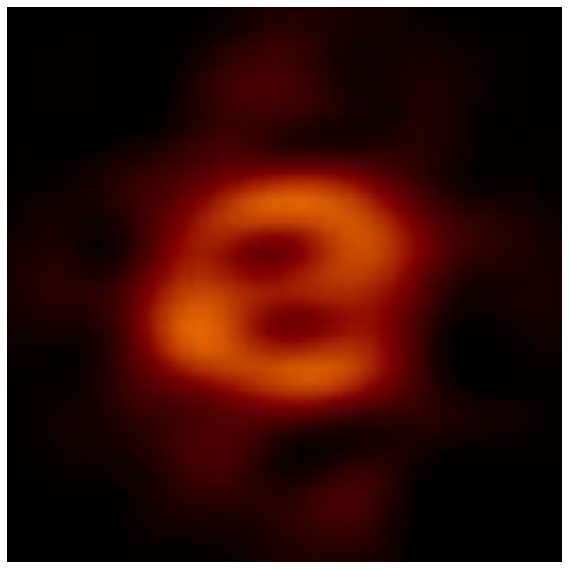
\includegraphics[height=.2\linewidth]{figures/propcmp/nomotion_NOPROP_hotoka02_vis_eht2017/mean_111.pdf} &
			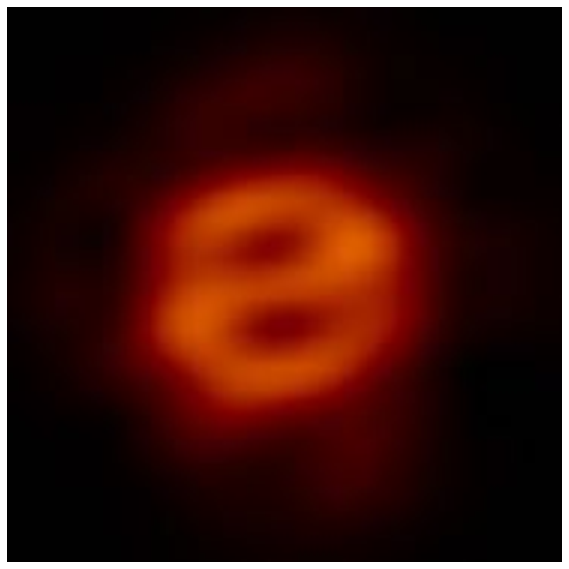
\includegraphics[height=.2\linewidth]{figures/propcmp/nomotion_NOPROP_hotoka02_vis_eht2017/mean_159.pdf} 
			\\
			\multirow{1}{*}[0.55in]{ \rotatebox[origin=t]{90}{\small{\textsf{NO ATM. }} }} \hspace{-0.25in} &
			\multirow{1}{*}[0.5in]{ \rotatebox[origin=t]{90}{\small{\textsf{ \& PROP.}} }} &
			{{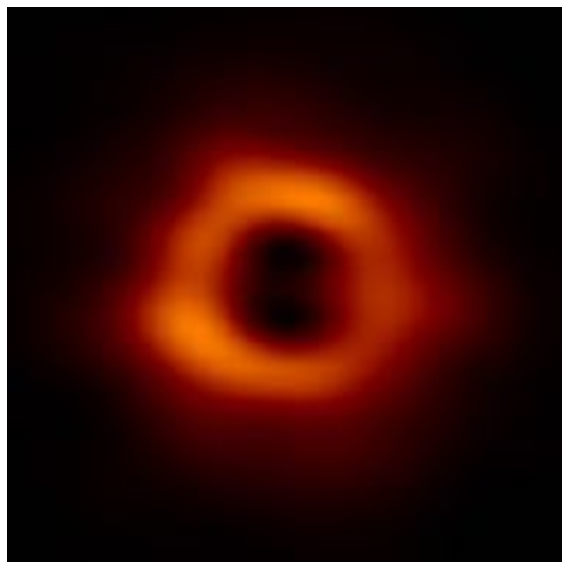
\includegraphics[height=.2\linewidth]{figures/propcmp/nomotion_ORIG_hotoka02_vis_eht2017/mean_74.pdf}} } &
			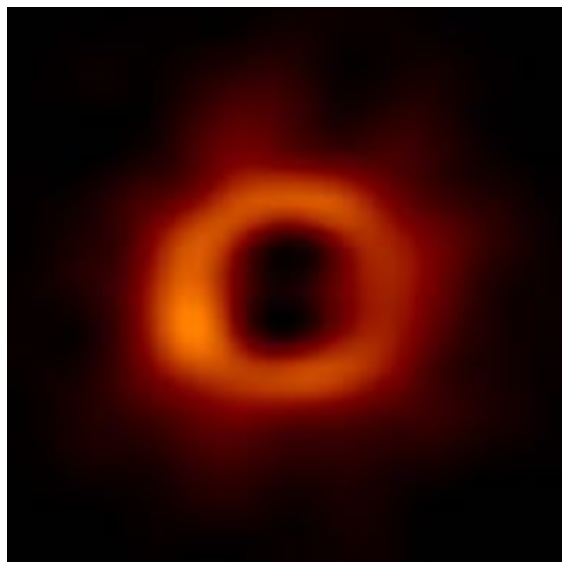
\includegraphics[height=.2\linewidth]{figures/propcmp/nomotion_ORIG_hotoka02_vis_eht2017/mean_111.pdf} &
			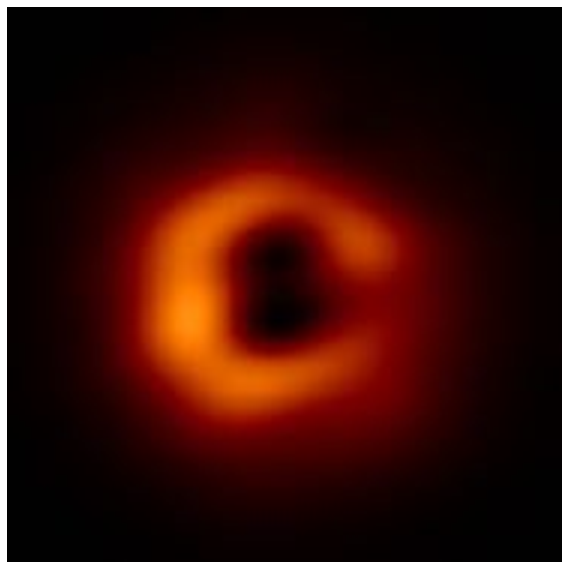
\includegraphics[height=.2\linewidth]{figures/propcmp/nomotion_ORIG_hotoka02_vis_eht2017/mean_159.pdf} 
			\\ \hline
			&\vspace{-.1in} & & & \\
			\multirow{1}{*}[0.45in]{ \rotatebox[origin=t]{90}{\small{\textsf{ATM. \&}} }} \hspace{-0.25in} &
			\multirow{1}{*}[0.55in]{ \rotatebox[origin=t]{90}{\small{\textsf{NO PROP.}} }}
			&
			{{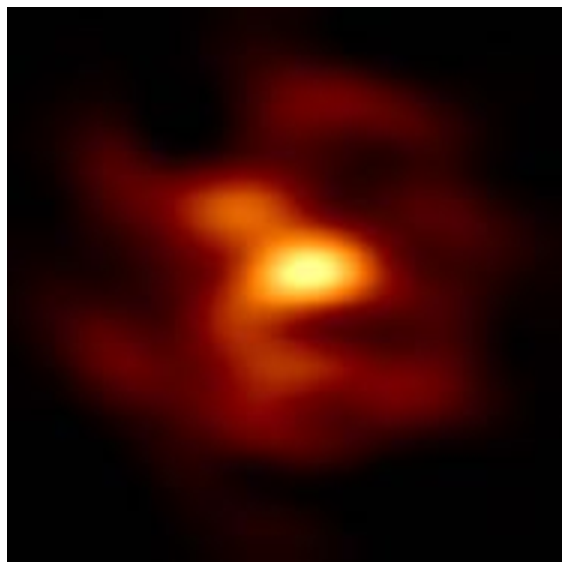
\includegraphics[height=.2\linewidth]{figures/propcmp/nomotion_NOPROP_hotoka02_ampbis_eht2017/mean_74.pdf}} } &
			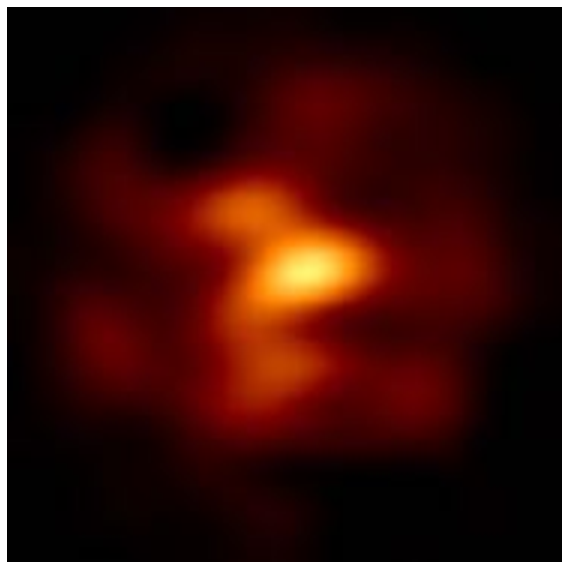
\includegraphics[height=.2\linewidth]{figures/propcmp/nomotion_NOPROP_hotoka02_ampbis_eht2017/mean_111.pdf} &
			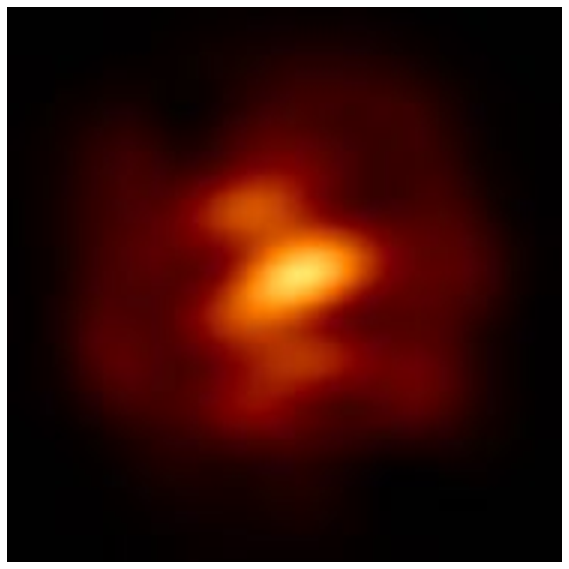
\includegraphics[height=.2\linewidth]{figures/propcmp/nomotion_NOPROP_hotoka02_ampbis_eht2017/mean_159.pdf} 
			\\ 
			\multirow{1}{*}[0.48in]{ \rotatebox[origin=t]{90}{\small{\textsf{ATM. \&}} }} \hspace{-0.25in} &
			\multirow{1}{*}[0.45in]{ \rotatebox[origin=t]{90}{\small{\textsf{PROP.}} }} &
			{{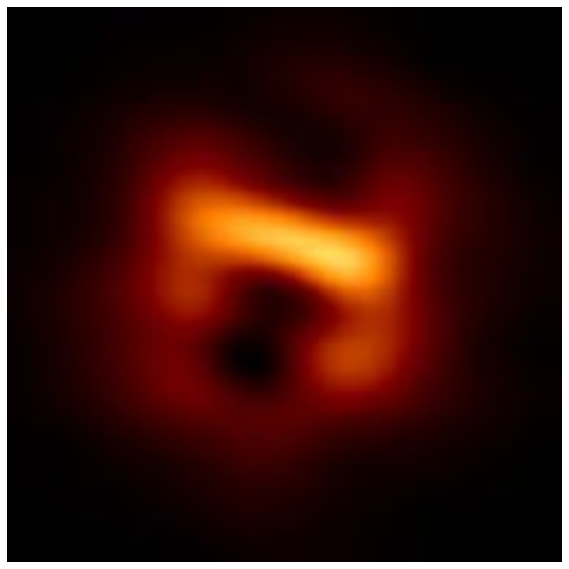
\includegraphics[height=.2\linewidth]{figures/propcmp/nomotion_ORIG_hotoka02_ampbis_eht2017/mean_74.pdf}} } &
			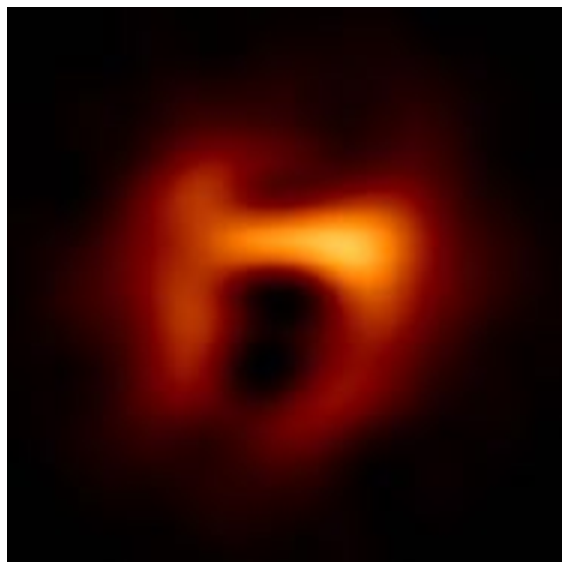
\includegraphics[height=.2\linewidth]{figures/propcmp/nomotion_ORIG_hotoka02_ampbis_eht2017/mean_111.pdf} &
			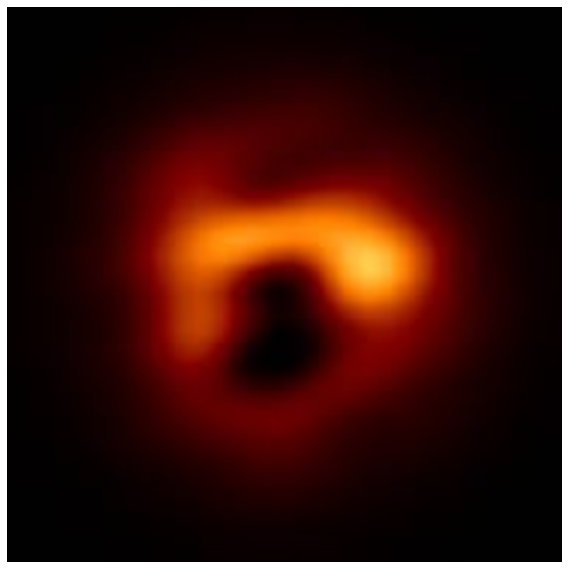
\includegraphics[height=.2\linewidth]{figures/propcmp/nomotion_ORIG_hotoka02_ampbis_eht2017/mean_159.pdf} 
			\\ \hline
		\end{tabular}
		\caption{{\bf Propagating Uncertainty:} During inference, StarWarps approximates each image's covariance matrix in order to propagate its uncertainty to neighboring frames in time. Propagating this information is crucial when using very few measurements. We show frames resulting from the same EHT2017 data of Video 3 when the covariance is propagated (PROP.) as described in this paper, versus not propagated (NO PROP.). Note that propagating the covariance results in significantly improved results. This is true even in the case of using non-linear measurements when atmospheric error is present (ATM.). In this non-linear case the covariance matrix is simply a crude approximation of the uncertainty, but proves critical in obtaining a result that captures the ring structure of the underlying source.   }
		\label{fig:propinfo}
	\end{center}
	\vspace{-.3in}
\end{figure}